\chapter{Method and Implementation}

This chapter outlines the work process for this study, designing a methodical approach to investigate emotions in Swedish speech using both AI-based analysis and self-reported data. The chapter describes the study’s approach and design, justifies methodological decisions, provides details regarding data collection and analysis procedures, and addresses validity and reliability considerations. 

\section{Approach and design}
This study adopts an explanatory sequential mixed method approach, which integrates both quantitative and qualitative approaches in a structured sequence. The study first collects and analyzes quantitative data, as AI-generated emotion labels and self-reported emotions, and then qualitative interprets the results to explore alignment and divergence. This approach ensures a systematic, layered analysis rather than pure comparison \autocite{Creswell2023}.  

The study follows a deductive research approach, as it builds upon existing theories of emotional expression in text and speech. The AI models will be tested and compared to established findings. Instead of developing new theories, the study aims to evaluate whether AI-based emotion recognition methods align with each other, prior research on vocal emotion markers and self-reported emotions for Swedish speech. 
This is classified as an experimental study, as it involves a controlled setting where participants are asked questions on predefined emotional recall scenarios. It does not manipulate independent variables in a traditional experimental way \autocite{Creswell2023}, instead observes and analyzes the natural emotional responses provoked through structured questions \autocite{Bryman2022}.

The study evaluates AI-generated emotion labels from speech compared with existing research on vocal markers, text-based emotion recognition and self-reported emotions. The self-reports serve as a reference point and not a ground objective truth, to acknowledge the subjective nature of emotional perception.  

\section{Data Collection}
The study involves participants for semi-structured interviews where they respond to predefined scenarios to provoke emotions. 
Ethical considerations, such as informed consent and anonymization, are followed firmly to ensure participant well-being. In the first phase, interviews are collected for analysis. 

16 Swedish speakers, primarily acquaintances to the researchers, are recruited via invitations. Interviews include 2 scenarios, 
each scenario includes 5-7 questions designed to elicit either positive or negative emotions, the participants select one of these questions for each semantic area, to maintain freedom in the speech as well as avoiding asking questions the participant are not comfortable to answer. The participants are not pre-informed about the feeling that are aimed to be provoked during the interviews. 
The scenarios have been pilot-tested for effectiveness. 
The interviews are recorded in a quiet room. Each scenario last between 2 and 4 minutes with breaks between them, the order of the scenarios varies to minimize affecting the results because of the possibility of the order influencing the different emotions. Each recording have been edited to delete our questions and any longer silent pauses. 

Participants are asked open-ended questions designed to bring out previously lived through personal experiences of anger and happiness. The questions about anger are focused on previous experiences of unfair treatment and frustration regarding their everyday lives or society, while the questions related to happiness explore moments of pride and unexpected joy through memories. 
The semi-structured format allows for follow-up questions based on participant responses, to bring out as much emotion as possible. The follow-up questions include "How did that make you feel?", "Can you evaluate on that specific situation?", and "What feelings did you experience?". See Appendix~\ref{list:prompts} for the full list of interviews. 

Audio is recorded and pre-processed to reduce background noise and normalise volume. Vocal markers from each recording are extracted using Parselmouth, a Python library for vocal feature extraction, to answer RQ1. The audio is analysed simultaneously using two emotion recognition models: Hume.ai to extract speech-based emotional labels, and NLP Cloud to transcribe the speech and then analyse the textual content in terms of emotion scores. The same dataset is used for all research questions to ensure consistency. 

The diagram in Figure~\ref{fig:pipeline} visualizes the multi-modal pipeline used in this study.  
The interview audio files are processed through three primary channels: speech-to-text transcription via NLP Cloud,  
Speech emotion recognition via Hume AI and acoustic feature extraction via Praat.  
These channels represent two main pipelines.  
The entities presented in yellow are prevalent in both pipelines, where the audio recordings are analyzed with Hume AI, the output is filtered to the 6 emotions analyzed in this study.  
The pipeline illustrated in green represents the analysis to answer research question 1.  
The vocal features extracting utilizing Praat Parselmouth are chosen are based on previous research, see \ref{sec:vocal-markers}, Theoretical Framework - Vocal Markers, where pitch, intensity/loudness, formant frequencies (F1, F2, F3), HNR,  
jitter and shimmer have distinguished values for certain emotions.  
To compare the extracted data with Hume AI, these values are clustered into emotion groups.  
Data from speech analysis and vocal markers are combined to statistically analyze the results for RQ1.  
The pipeline used to answer the second and third research question is presented in orange. 
Interview audio is processed the same way as for RQ1 but extended with normalization for the Hume values to enable comparison with outputs from NLP Cloud and self-assessment.  
For text-based emotion recognition, the recording is transcribed before text-analysis is composed. 
Results from speech and text prediction are combined with the self-assessment scores to answer RQ2 and RQ3. 

\begin{figure}[H]
    \centering
    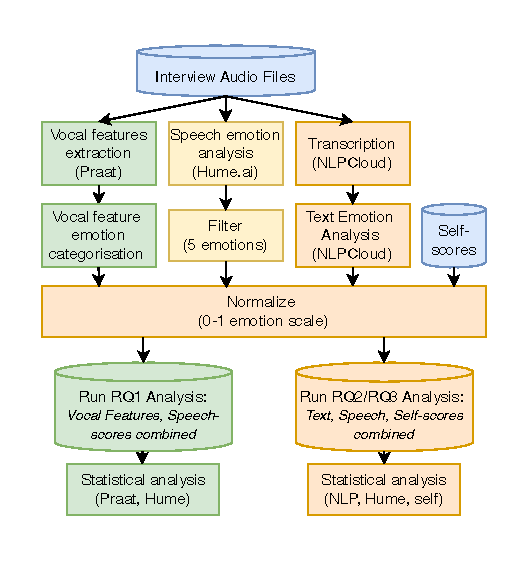
\includegraphics[width=0.8\textwidth]{png/method/flowchart-thesis.pdf}
    \caption{The multi-modal pipeline used in this study.}
    \label{fig:pipeline}
\end{figure}


\subsection{Research Question 1}
\textbf{How does AI-model for speech emotion recognition compare to research on vocal markers for emotions in Swedish speech?}

To answer this question, speech recordings are collected from participants as they describe emotionally charged experiences. AI-based emotion recognition using Hume.ai, are used for AI-based Speech Emotion Recognition. Voice feature extraction from the recordings is made, to compare to AI-labeled emotions with known vocal markers from existing Swedish emotion research \autocite{Ekberg2023}. 

\subsection{Research Question 2}
\textbf{What similarities and differences emerge between emotions detected from audio features and from the textual transcripts of the same speech data?}

To answer the second question, the recorded speech is transcribed and analyzed for emotion recognition using NLP Cloud’s emotion recognition to assess the emotional content of speech transcripts. The text-based AI labels are compared with speech-based AI labels to determine whether emotion is preserved in textual content alone. 

\subsection{Research Question 3}
\textbf{How do AI-generated emotion labels (speech \& text-based) compare to self-reported emotions? }

For the third question, participants complete a self-assessment survey after each interview segment, where they rate their emotional state on a 1-6 scale (1 = very weak, 6 = very strong) for relevant emotions. The self-reported emotions are compared with AI-generated labels from both speech and text models to analyze agreement and divergence. The results are clustered as agreements, partially agreements, and disagreements across methods. 


\section{Data Analysis}
\label{sec:method-data-analysis}
To systematically evaluate the agreement between different emotion detection methods, a combination of statistical analyses and visualizations was applied for speech-based AI, text-based AI, vocal markers, and self-reported emotions. 
The analysis aimed to assess the alignment with established vocal marker research and subjective human perception, where identification and categorization of differences where analyzed. 

Visualised analysis is included as a complement to tables with data, for easy interpertation of how the different methods correlate and observe behavioral differences, or where the models agree. 
This includes correlation heatmaps, confusion matrices of top emotion labels, scatter plots illustrating two methods mean emotion probability, and bar charts. 
Individual clips are presented with bar charts and diagrams representing changes over time segments. 



\subsection{Emotion Categorization from Vocal Markers}
\label{sec:method-data-an-voc}
We analysed each of the 30 clips in several stages to answer the first research question. Extracted vocal features included mean pitch (st, Hz), mean intensity(dB), mean hnr (dB), F1, F2, F3 formants (Hz), jitter and shimmer see Theoretical Framework~\ref{sec:vocal-markers}.
First, acoustic features were categorized in five emotion groups based on standardized distances based on Table~\ref{fig:compare-acoustic-parameters}. Because of the method yielded near uniform emotion scoring (≈0.20), a rule-based function was developed and refined through four variants (V0-V3), 
where threshold adjustions and anchors was applied to each layer. 

\subsubsection{Standardized distance function}
\label{sec:method-stand-func}
\begin{itemize}
    \item 1. Predefined means and standard deviations for each vocal features identified for each emotion were retrieved from the Swedish research \autocite{Ekberg2023}. These features are stored in JSON format. 
    \item 2. For every feature included in a recording, the function calculates the standardized distance between the measured vocal value and the mean for each emotion: 
    \[
    d_{\text{emo}} \, \text{+=} \, \frac{|x - \mu|}{\sigma}
    \]
    where \( x \) is the observed value, and \( \mu \), \( \sigma \) are the mean and standard deviation for the pair of feature and emotion.  
    \item 3. To increase the functionality, distances are inverted so smaller distances can result in higher emotion scores. 
    This is calculated with the function below, where \( \epsilon \) is a small constant to avoid division with zero. 
    \[
    \text{score}_{\text{emo}} = \frac{1 / (d_{\text{emo}} + \epsilon)}{\sum_{e} 1 / (d_{e} + \epsilon)}
    \]
    \item 4. The output is a normalized probability value that is distributed across all five emotions. 
\end{itemize}
Baseline for neutral speech was not described in the reffered research, therefore the baseline for this study is the average vocal features of all clips. 
Analysis of our data yielded every emotion probability around 0.18-0.22 for each clip, appearing creating arbitrary scores. This motivated the rule-based approach. 

\subsubsection{Rule-based method: V0 (Global K)}

To mark outer values, 90\% confidence interval were used to mark the outer population \autocite{Bruce2017} yielding the critical value Z = $\pm$ 1.645 $\sigma$. 
Our threshold K\_EXTREME was therefore initialized to 1.6 $\sigma$ for all emotions. For the normal distribution range we used roughly 1.5 standard deviation from mean, as K\_NEAR = 1.25 $\sigma$. 
Benchmarks from \textcite{Ekberg2023} were applied: 
\begin{itemize}
    \item "anger": [("hnr","below"), ("jit","below"), ("loud", "above")]
    \item "joy": [("pitch","above"), ("hnr","above"), ("loud","above")]
    \item "sadness": [("pitch","below"), ("hnr","below"), ("loud", "below")]
    \item "fear": [("hnr","above"), ("jit","below")]
    \item "surprise": [("jit","above"), ("shim","above")]
\end{itemize}
If any emotion goes beyond the extreme threshold, the emotion is scored. 

For all eight features, if the clip value is within the K\_NEAR, 1.25 $\sigma$ of an emotion's mean, one more point is added, to ensure typical matches are added even if no extreme cue is found. 

After the functions loop, each emotion has a score and the highest score is assigned the clip's main emotion label. 

V0 resulted in mainly anger and surprise scores. 
\subsubsection{Rule-based method: V1 (Per-emotion K)}
K\_EXTREME values were adjusted for all emotions. Justifications is described in Theoretical Framework~\ref{sec:vocal-markers} explaning wide spread acoustic pattern for happiness and similar vocal palette as anger. 
Therefore, joy was set to a smaller extreme value while heightened for anger. 
Joy = 0.5 $\sigma$ 
Anger = 1.6 $\sigma$ 
Others = 1.0 $\sigma$

\medskip
V1 showed the same results as V0 with no distinct difference. 

\subsubsection{Rule-based method: V2 (+ Feature Weight)}
V1 was extended with utilizing the standardised function \ref{sec:method-stand-func} as fallback before returning the loaded dictionary with emotion scores. 
The returned values from the standardised function was multiplied with 0.25 and added to the rule-based versions result.

Initially, all vocal features were equally weighted as 1.0. For this version, loudness were decreased to 0.5 motivated by prior research showing that loudness is the 
least discriminative of the vocal features extracted for this study as explained in \ref{sec:vocal-markers}. 

The approach yield more dispered emotion scores but still rated anger as top-label for more than 50\% of the recordings. 

\subsubsection{Rule-based method: V3 (+ Benchmarks)}
Benchmarks cues for anger, joy, and sadness was implemented to avoid overlabeling. To yield a score, anger are required to have at least two benchmark cues, ensuring at least two of the emotion-specific benchmarks (see V0) is fulfilled.  
Joy and sadness need one of their individual benchmark. This approach avoids false scoring. 

Other emotions skip this gate and can only get their scores from their seperate benchmarks. Each score is worth 1.0 points. 

This gating is motivated by data from \textcite{Ekberg2023}, see Theoretical Framework~\ref{sec:vocal-markers}, showing that pitch and intensity are most distinctive for 
the two high-arousal emotions, while single universal cues caused possibly misjudged positives in the pilot runs Results~\ref{rq1_pilot_tests}. The affected clips were analysed seperately and compared to Table~\ref{fig:compare-acoustic-parameters} for this conclusion. 

In this version, the individual extreme values, k, was tested and changed to 1.0 for all except joy, changed to 0.7. This did not affect the results. 
Version 3 is the final method that is used for data analysis in results. The full code is listed in Appendix~\ref{lst:categorise_emotion}.

\subsubsection{Analysis rule-based emotion categorisation and Hume AI}
Alignment and divergence between the rule-based function and Hume AI emotion probability is analysed with confusion matrices including both sources top-label for each interview. 
Mean rating score for the full dataset is visualised with scatter plots followed by Pearson's correlation coefficients to assess relationships and corresponding significance. 

\subsubsection{Comparison Hume and Vocal Features}
Analysis that are not including the emotion categorisation function includes the following vocal features: Pitch, Loudness/Intensity, HNR, Shimmer, and Jitter. To explore the relationship between Hume AI Emotion labels and vocal features, without feature based emotion categorisation, further analysis were conducted to assess correlation between each acoustic marker and Hume predefined emotions, presented as a heatmap.
Further analyses include one-way ANOVA tests, see \ref{sec:theo-stat-analyse} for clarification. 
To track patterns over time and enable more detailed analysis, each audio recording were segmented into timeframes including Hume AI emotion scoring and vocal features for that specific segmment. These were analyzed by tracking Z-score variations, see \ref{sec:theo-stat-analyse}, in key vocal features (pitch, intensity, jitter, and shimmer) throughout each recording.
The general time-segment is set to 1.25 seconds. For case examples \ref{sec:res_rq1_case}, different time-segments were tested to observe correlation differences depending on segment length for executed vocal analysis. 
Beside correlation measurements, top 30\% and bottom 70\% of emotion probability time-segments are compared to test wheather the mean z-scored feature differs between the high vs. low groups. 
A large t-statistic value indicate a reliable shift in that feature when Hume rates that emotion high. For the time-segmented analysis, the baseline was set to the average vocal value for our dataset. 

Output from Hume AI include segmented results with individual time stamps, varying for each clip. Vocal feature extraction is set to a fixed 1.25s window, therefore, the segments are not fully aligned. 
By this reason, individual recordings from two interviews are included to visualise how pitch and intensity behaves for Hume labelled joy and sadness. 

\subsection{RQ2 and RQ3: Speech-Based AI vs. Text-Based AI, AI-labels vs. Self-Assessed Emotions}
For both RQ2 and RQ3, statistical analyses were used to evaluate the alignment between AI-generated emotion scores and self-reported emotions. The following methods were applied across both research questions:
\begin{itemize}
    \item Pearson correlation coefficients and associated p-values for measurement both for single clips and the full dataset. 
    \item T-tests and calculation of Cohen's d to evaluate statistical significance and effect sizes. 
\end{itemize}
For all statistical tests, a p-value below 0.05 was considered as statistical significant, implying that the observed correlations or differences were unlikely to have occurred by chance. 
These statistical methods were applied to the entire dataset, and separately for negatively and positively oriented interview scenarios to identify potential contextual differences.
For RQ2, comparisons focused on speech-based vs. text-based AI results, and RQ3 extended the comparison to include self-reported emotions as a subjective component.

\subsection{Data Normalization}
To enable direct comparison across different sources, all emotion scores were normalized to sum up to 1. The normalization included the following steps: 
\begin{itemize}
    \item 1. Surprise combination: Hume AI predicted two seperate labels for Surprise, one positive and one negative. These were merged into a single "surprise" by calculating the average. 
    \item 2. Filtering and formatting: Filtering to only include the five target emotions (anger, joy, sadness, fear, surprise), since Hume predicted around 30 different emotions. All emotion labels were converted to lowercase. 
    \item 3. Normalization: The emotion scores were normalized so the sum of all five target emotion values equals 1. This was done by dividing each score by the total sum of the emotion values. If the total sum was zero (no emotion detected), all scores were set to 0. 
\end{itemize}
Normalization ensured consistent comparability between the sources, for both AI models and self-assessments, regardless of scale differences in raw scores. 
\subsection{Visual Analysis}

To evaluate the performance of the custom vocal feature-based emotion categorization method, line plots and bar charts were implemented to visualize differences between the generated scores and Hume AI's predictions. 
The line plot summerizes average emotion scores across the full dataset, while bar charts presented detailed comparisons for individual audio recordings. 
These diagrams emphasizes deviations and alignments between the categorized vocal marker method and AI-based emotion prediction. 

Composite correlation diagrams were used to explore associations between single vocal features and AI-generated emotion scores. 
For these diagrams, Pearson correlation coefficients were calculated for each emotion and its relation to pitch and intensity, the results are visualized as grouped bar charts to easily identify positive or negative tendencies. 

Visualizations were also integrated to support the identification of alignment patterns between the AI systems, and contributed with insights into how the modality of the AI influences emotion recognition results. 
Python have been utilized to create all visualizations. 

Given the limited dataset size and timeframe, a combination of statistical methods and visual analysis, was utilized to balance quantitative data with qualitative interpretation and support the exploratory nature of this study. 

\section{Model Configuration}
\subsection{NLP Cloud}
\label{sec:method-nlp}
The text-based emotion recognition is classified with NLP Clouds finetuned-llama-3-70b model
through prompting, which allows a more flexible approach.
Each text input uses the following prompt:
\begin{center}
    \begin{minipage}{0.7\textwidth} 
    \begin{lstlisting}[language=json, caption={NLP Cloud configuration prompt.}]
prompt = (
"You are an emotion analysis system.
Given a Swedish text, respond only with a JSON object using these emotion labels: 
joy, surprise, fear, anger, sadness.
Each value must be a float between 0.0 and 1.0.
Respond with the JSON directly and nothing else.
f"{transcription}"
)
    \end{lstlisting}
    \end{minipage}
\end{center} 
The prompt that is used returns a JSON response with float values ranging from 0.0 to 1.0 for each of
the emotions with the labels “joy”, “surprise”, “fear”, “anger”, “disgust” and “sadness”. This approach
was chosen to ensure these specific emotions being analyzed due to them being the feelings of the basic
six, which are the feelings used in the research about acoustic features in swedish speech done by
Ekberg \autocite{Ekberg2023}. 

\subsection{Hume AI}
To ensure consistency across the different models used in this research, some changes have been
made to adjust the output from the Hume AI model to better match the format used in NLP Cloud.
Additionally, NLP Cloud has the feeling surprise while Hume has two different feelings for surprise,
the two being positive surprise and negative surprise. Therefore, the scores of the two feelings of
surprise from the Hume model have been combined in this research to give just one number that
creates the average of the two to match the format.

\section{Validity and Reliability}
\subsection{Validity}
To ensure validity, the interview scenarios are pilot tested to ensure they provoke intended emotions \autocite{Bryman2022}. The use of multiple AI models (speech- and text-based) allows for cross-validation of results. Standardized interview prompts ensure consistency across participants. Participant self-assessment serves as a secondary reference to evaluate AI-labeled emotions. Triangulation across AI, vocal markers, text analysis, and self-assessments enhance convergent validity \autocite{Creswell2023}. 

\subsection{Reliability}
To ensure reliability, standardized equipment and scenario are used to ensure replicability. Hume.ai, NLP Cloud, and Praat provide consistent measures. The AI models used in the study (Hume.ai and NLP Cloud) are pre-trained and validated emotion recognition systems. Correlation will be determined and are used to quantify the reliability of AI models in detecting emotions. 
The same data is not analysed multiple times to check if the results are different. The prompt used for NLP Cloud is therefore zero-shot. 
The study has a replicable experimental setup, with documentation supporting replication to allow researchers to reproduce similar evaluations.  

Triangulation is achieved in the study through comparison of speech AI, text AI, and self-reports which improves creditability. Any discreteness will be analyzed qualitatively to contextualize potential biases rather than assuming errors. 
Reliability is ensured through standardization in data collection. All interviews are preprocessed to reduce background noise and normalize volume levels. The online tool Auphonic \autocite{Auphonic} is used for this, due to its simple usability for noise reduction, ability to cut out pauses and limit loudness. The same data processing steps are applied consistently for all recordings, ensuring equality in analysis. The study has a replicable experimental setup, with usage of pre-trained, publicly available APIs, and documentation supporting replication to allow researchers to reproduce similar analyses. These measures ensure that our study is generalizable within the scope or automated emotion recognition for stress analysis. 

\section{Considerations}
To consider the implications of this study, several factors must be recognized. To address ethical and privacy concerns, all participant data is anonymized and securely stored to ensure privacy. The participants provide informed consent before engaging in this study. The emotion-provoking scenarios are designed to minimize distress, focusing on natural, everyday emotions rather than triggering events. The participants will have scenarios to choose from, see 2.2 Data Collection. 

Scientific considerations extend to emotion research to Swedish speech and AI tools. Findings in the study can inform future human-interaction research in emotion-based applications. Societal considerations include that the insights could enhance AI-driven mental health tools and future research, especially for Swedish language and real-world interviews. 
